\documentclass[10pt,a4paper]{article}
\usepackage{amsmath,amssymb,amsthm,graphicx}
\usepackage[no-math]{fontspec}
\usepackage{graphicx,amsmath,amssymb}
\newenvironment{authorclaim}[1]{\par\medskip\noindent\textbf{#1.}\ }{\par\medskip}
\allowdisplaybreaks
\title{Majority composition in randomised query complexity with expected small-error inner cost}
\author{Mika Göös, Gilbert Maystre}
\date{doi:10.4230/LIPIcs.CCC.2021.18; CC BY 4.0}
\begin{document}
\maketitle
\noindent\textit{Editorial scope.} Counted once: complete majority-lemma result, incorporating general GapOr reduction and every source-local leaf/abort/minimax support argument. Worst-case R and expected bar-R costs, partial domains and all error conventions remain distinct as authored. No separate count for hard sides, parameter ranges, GapOr reduction or support lemmas.\par\medskip
\noindent\textit{Allowed standard prerequisites (editorial).}\begin{itemize}
\item Partial-function decision trees, conical juntas, imported direct-sum/nonnegative GapOr bounds and abort-tree minimax. Exact original definitions and imported [5, Theorem4], [7] direct-sum and Lemmas8/9 retained. All source-local error reduction, Simulation, Leaf, HardSide and Multileaf proofs included. Full25 published references. Imported independent-paper proofs not recursively reproduced.
\end{itemize}\medskip
% Faithful formal-publication transcription of the main statements and necessary query-model definitions.
\section*{Author result and reduction}
We assume $n\ge3$ for simplicity of notation throughout the paper.

\begin{authorclaim}{Theorem2 (Maj lemma)}
$R(\mathrm{Maj}\circ g^n)=\Theta(n\cdot\overline R_{1/n}(g))$ for every partial function $g$.
\end{authorclaim}

Previously, Ben-David et al. [5] proved Theorem2 in the special case $g=\mathrm{GapOr}$. Here $\mathrm{GapOr}=\mathrm{GapOr}_m$ is the $m$-bit partial function defined by $\mathrm{GapOr}(x)=\mathrm{Or}(x)$ on inputs of Hamming weight $|x|\in\{0,m/2\}$ and is undefined otherwise. This is a particularly clean example of a function whose query complexity behaves as (assuming $m\ge\log(1/\epsilon)$)
\[\overline R_\epsilon(\mathrm{GapOr})=\Theta(\log(1/\epsilon)).\]
We prove Theorem2 by a direct reduction to this previous result! Our more general result says, informally, that error reduction is necessary for any composed function $f\circ g^n$ if it is necessary in the special case $g=\mathrm{GapOr}$. Our key conceptual insight is to formulate a sense in which every $g$ can be ``simulated'' by GapOr. There is, however, a slight technical caveat. For the reduction to work, we need to assume that the lower bound for $f\circ\mathrm{GapOr}^n$ holds not only against randomised decision trees but also against a more powerful model called $\epsilon$-approximate nonnegative degree $\deg^+_\epsilon$ (aka conical junta degree, partition bound), which we will recall in Section2.
\begin{authorclaim}{Theorem3 (Reduction to GapOr)}
If a function $f$ satisfies $\deg^+_\epsilon(f\circ h^n)\ge\Omega(n\log n)$ for some constant $\epsilon>0$ and for both $h\in\{\mathrm{GapOr}_{\log n},\neg\mathrm{GapOr}_{\log n}\}$, then
\[\forall g:\quad R(f\circ g^n)=\Omega(n\cdot\overline R_{1/n}(g)).\]
\end{authorclaim}
Theorem2 follows immediately by combining Theorem3 with [5, Theorem4], which proved the required nonnegative degree lower bound for $\mathrm{Maj}\circ\mathrm{GapOr}^n$ (we only note that their proof works equally well for $\neg\mathrm{GapOr}$ in place of GapOr). In fact, the nonnegative degree lower bound holds more generally for any $(2n+1)$-bit outer function that agrees with Maj on inputs of weight $n$ and $n+1$. For example, Xor is such a function, and hence the Xor lemma of Brody et al. [8] can be recovered using Theorem3. However, the original proof in [8] is much simpler than ours, and moreover, the result of [8] actually characterises $\overline R_\epsilon(\mathrm{Xor}\circ g^n)$ for all $\epsilon>0$ while we focus on the bounded-error case $\epsilon=1/3$.
Our goal for the rest of the paper is to prove Theorem3.
For randomised query complexity, a complete answer [to the direct sum problem] was recently obtained by Blais and Brody [7] (improving on [17,6]). Their result states
\[\forall g:\quad R(g^n)=\Theta(n\cdot\overline R_{1/n}(g)).\tag{Direct sum}\]
\section*{2 Query complexity basics}
We study partial boolean functions $f:\{0,1\}^n\to\{0,1,*\}$. The domain of the function is $\operatorname{dom}(f):=f^{-1}(\{0,1\})$ and the inputs $f^{-1}(*)$ are undefined. We say $f$ is total if $\operatorname{dom}(f)=\{0,1\}^n$. For partial functions $f$ and $g$, their composition $f\circ g^n$ is defined by $(f\circ g^n)(x_1,\ldots,x_n):=f(g(x_1),\ldots,g(x_n))$ if $x_i\in\operatorname{dom}(g)$ for all $i\in[n]$; otherwise $(f\circ g^n)(x_1,\ldots,x_n):=*$. Standard references for boolean function complexity are [9,18].
\paragraph{Decision trees.} A (deterministic) decision tree $t$ is an algorithm for computing a boolean function on an unknown input $x\in\{0,1\}^n$. The algorithm repeatedly queries the input variables $x_i\in\{0,1\}$ in some order (which can depend on outcomes of queries made so far) until eventually producing an output $t(x)$. Such an algorithm can be represented as a binary tree, with internal nodes labelled with variables $x_i$, outgoing edges of the internal nodes labelled with query outcomes ($x_i=0$ and $x_i=1$), and leaves labelled with output values. Each input $x$ determines a unique root-to-leaf path, obtained by following the query outcomes consistent with $x$. The most important cost measure of $t$ is its depth, denoted $\operatorname{depth}(t)$, which is the longest root-to-leaf path in the tree and equals $\max_xq(t,x)$ where $q(t,x)$ denotes the number of queries made by $t$ on input $x$.
A randomised decision tree $T$ is a distribution over deterministic decision trees $t\sim T$. We say $T$ computes $f:\{0,1\}^n\to\{0,1,*\}$ with error $\epsilon$ if for every $x\in\operatorname{dom}(f)$ we have $\Pr_{t\sim T}[t(x)=f(x)]\ge1-\epsilon$. There are two cost measures for $T$: the (worst-case) depth is the maximum depth of any decision tree in the support of $T$; the expected depth is $\max_x\mathbb E_{t\sim T}[q(t,x)]$. The $\epsilon$-error query complexity of $f$, denoted $R_\epsilon(f)$, is the least depth of a randomised decision tree that computes $f$ with error $\epsilon$. The $\epsilon$-error expected query complexity, denoted $\overline R_\epsilon(f)$, is defined analogously.
\paragraph{Error reduction.} It is well known that the error probability of an algorithm (computing a boolean-valued function) can be reduced from any constant $1/2-\delta$, where $\delta>0$, to any other constant $\epsilon>0$ by repeating the algorithm constantly many times (in fact, $O(\log(1/\epsilon)/\delta^2)$ many) and outputting the majority answer. Hence we often set $\epsilon:=1/3$ and omit $\epsilon$ from notation. In this bounded-error regime, we have $\overline R(f)\le R(f)\le O(\overline R(f))$ where the second inequality follows by truncating executions that query many more bits than the expectation. For vanishing $\epsilon=o(1)$ (as $n\to\infty$), it is possible that $\overline R_\epsilon(f)\le o(R_\epsilon(f))$. For example, consider the partial $2n$-bit function $f$ where the task is to distinguish inputs of the form $x0^n$ from inputs of the form $0^nx$ with the promise that $|x|=n/2$. We have $\overline R_{1/n}(f)=O(1)$ while $R_{1/n}(f)=\Theta(\log n)$. In this small-error regime, the following fine-grained error reduction calculation will be useful.
\begin{authorclaim}{Claim7}
$\overline R_{\epsilon^k}(f)\le4k\cdot\overline R_\epsilon(f)$ for every $k\ge1$ and $\epsilon\le1/16$.
\end{authorclaim}
\begin{proof}
Suppose $T$ computes $f$ with error $\epsilon$ and consider the algorithm $T'$ that runs $T$ $4k-1$ times and outputs the majority answer. Then $T'$ errs iff at least $2k$ of the runs err. This happens with probability at most $\sum_{i=2k}^{4k-1}\binom{4k-1}i\epsilon^i(1-\epsilon)^{4k-1-i}\le2^{4k}\epsilon^{2k}\le\epsilon^k$.
\end{proof}
\paragraph{Leaf indicators.} Let $t$ be a decision tree with $n$-bit inputs. We denote by $L(t)$ the set of its leaves and by $\ell_x^t\in L(t)$ the unique leaf reached on input $x$. We often identify a leaf $\ell\in L(t)$ with its associated leaf indicator function $\ell:\{0,1\}^n\to\{0,1\}$ defined by $\ell(x):=1$ iff input $x$ reaches leaf $\ell$. Thus each $\ell$ is simply a conjunction of at most $\operatorname{depth}(t)$ literals ($x_i$ or $\overline x_i$) determined by the unique root-to-$\ell$ path in $t$. If $t$ outputs boolean values, we let $A(t)\subseteq L(t)$ denote the set of accepting leaves, that is, those that output 1. Since the leaf indicators have pairwise disjoint supports, we can write the function computed by $t$ as
\begin{equation}\tag{1}t(x)=\sum_{\ell\in A(t)}\ell(x).\end{equation}
\paragraph{Nonnegative degree.} Let $p:\{0,1\}^n\to\mathbb R_{\ge0}$ be a nonnegative function. We say $p$ is a nonnegative $d$-junta if it depends on at most $d$ of its variables. For example, if $t$ is a depth-$d$ decision tree, then each $\ell\in L(t)$ is a nonnegative $d$-junta. More generally, we say that $p$ is a conical junta of degree $d$ if it can be written as a conical combination of nonnegative $d$-juntas, that is, $p(x)=\sum_i a_iq_i(x)$ where $a_i\ge0$ are nonnegative scalars and the $q_i$ are nonnegative $d$-juntas. For example, the function computed by $t$ is a degree-$d$ conical junta, as given by the expression(1). The nonnegative degree of $p$, denoted $\deg^+(p)$, is the least $d$ such that $p$ is a degree-$d$ conical junta.
Let $f:\{0,1\}^n\to\{0,1,*\}$ be a partial function. We say that $p$ $\epsilon$-approximates $f$ if $p(x)\in f(x)\pm\epsilon$ for every $x\in\operatorname{dom}(f)$. The $\epsilon$-approximate nonnegative degree of $f$, denoted $\deg^+_\epsilon(f)$, is the least degree of a conical junta that $\epsilon$-approximates $f$. For example, if $T$ is a depth-$d$ randomised $\epsilon$-error decision tree for $f$, then there exists a degree-$d$ conical junta $p_T$ that $\epsilon$-approximates $f$, namely,
\[p_T(x):=\mathbb E_{t\sim T}[t(x)]\in f(x)\pm\epsilon.\]
This shows that $\deg^+_\epsilon(f)\le R_\epsilon(f)$. The gap betweeen $\deg^+_{1/3}(f)$ and $R(f)$ can be huge for partial functions. For example, consider the $n$-bit UniqueOr defined by $\mathrm{UniqueOr}(x)=\mathrm{Or}(x)$ for inputs of weight $|x|\in\{0,1\}$ and undefined othwerwise. Then $\deg^+(\mathrm{UniqueOr})=1$ (computed by $\sum_ix_i$) while $R(\mathrm{UniqueOr})=\Theta(n)$. For total functions, the gap is at most polynomial [9].
Nonnegative degree has been studied under many names: (one-sided) partition bound [16], WAPP query complexity [14,5], and query complexity ``in expectation'' [19].
\section*{Necessary Leaf and Multileaf Lemma definitions (Section3.1)}
For a leaf $\ell\in L(t)$ and any input distribution $\mu$ we write for short $\ell(\mu):=\mathbb E_{x\sim\mu}[\ell(x)]=\Pr_{x\sim\mu}[\ell(x)=1]$.
Fix a partial function $g:\{0,1\}^m\to\{0,1,*\}$. Let $\mu=\frac12(\mu^0+\mu^1)$ be a balanced distribution where $\mu^i$ is supported on $g^{-1}(i)$. For a leaf $\ell$ over $m$ bits, a ``hard side'' $b\in\{0,1\}$, and an error parameter $\epsilon\ge0$, we define
\[\ell\text{ is }(\epsilon,\mu,b)\text{-noisy}\quad\Longleftrightarrow\quad\ell(\mu^{1-b})\ge\epsilon\cdot\ell(\mu^b).\]
For simplicity of notation, for small quantities $a,b\in[0,1]$, we write $a\ll b$ (resp. $a\lll b$) to mean $a\le cb$ (resp. $a^c\le b$) for a sufficiently small constant $c>0$.
\begin{authorclaim}{Leaf Lemma}
For every partial $g$ and $0<\epsilon\lll\delta\ll1$, there exists a distribution $\mu=\frac12(\mu^0+\mu^1)$ over $\operatorname{dom}(g)$ and a hard side $b\in\{0,1\}$ such that for every deterministic tree $t$ and $i\in\{0,1\}$:
\[\frac{\mathbb E_{x\sim\mu^i}[q(t,x)]}{\overline R_\epsilon(g)}\lll\delta\quad\Longrightarrow\quad\Pr_{x\sim\mu^i}[\ell_x^t\text{ is }(\epsilon,\mu,b)\text{-noisy}]\ge1-\delta.\]
\end{authorclaim}
In order to use Leaf Lemma in the context of composed functions, we generalise it to the direct sum setting where the inputs come from $\operatorname{dom}(g^n):=\operatorname{dom}(g)^n$. Let $\ell$ be a leaf over $nm$ bits and write $\ell(x)=\prod_{i\in[n]}\ell_i(x_i)$ where $x_i\in\{0,1\}^m$ and each $\ell_i$ is over $m$ bits. We define
\[\ell\text{ is }(\delta,\epsilon,\mu,b)\text{-noisy}\quad\Longleftrightarrow\quad\ell_i\text{ is }(\epsilon,\mu,b)\text{-noisy for at least }(1-\delta)n\text{ many }i\in[n].\]
Our generalised lemma says that we will typically reach a noisy leaf if we run a shallow decision tree on a random input from the product distribution $\mu^y:=\mu^{y_1}\times\cdots\times\mu^{y_n}$ where $y\in\{0,1\}^n$.
\begin{authorclaim}{Multileaf Lemma}
For every partial $g$ and $0<\epsilon\lll\delta\ll1$, there exists a distribution $\mu=\frac12(\mu^0+\mu^1)$ over $\operatorname{dom}(g)$ and a hard side $b\in\{0,1\}$ such that for every deterministic tree $t$ taking inputs from $\operatorname{dom}(g^n)$ and having $\operatorname{depth}(t)/(n\overline R_\epsilon(g))\lll\delta$,
\[\forall y\in\{0,1\}^n:\quad\Pr_{x\sim\mu^y}[\ell_x^t\text{ is }(\delta,\epsilon,\mu,b)\text{-noisy}]\ge1-\delta.\]
\end{authorclaim}

% Faithful formal-publication transcription of complete Section3.2 proof.
\section*{3.2 Proof of Theorem3}
We conclude this overview section with a proof of Theorem3 using Multileaf Lemma. We start with a lemma that shows how the noisy leaves in the domain of $g^n$ can be ``simulated'' by low-degree conical juntas in the domain of $\mathrm{GapOr}^n$. For simplicity, we state the lemma assuming a hard side $b=0$; an analogous lemma holds for $b=1$ by replacing GapOr with $\neg\mathrm{GapOr}$.
\begin{authorclaim}{Simulation Lemma}
Let $\ell$ be a $(\delta,\epsilon,\mu,0)$-noisy leaf over the variables of $g^n$. There exists a conical junta $p_\ell:(\{0,1\}^{\log n})^n\to\mathbb R_{\ge0}$ of degree at most $n\cdot[\delta\log n+\log(1/\epsilon)]$ such that
\[\forall x\in\operatorname{dom}(\mathrm{GapOr}_{\log n}^n):\quad p_\ell(x)=\ell(\mu^{\mathrm{GapOr}_{\log n}^n(x)}).\]
\end{authorclaim}
\begin{proof}
We start by defining three conical juntas in the domain of $\mathrm{GapOr}_m$ for $m:=\log n$. Let $S_k^m$ be the distribution over multisets obtained by picking $k$ random elements from $[m]$ with replacement.
\begin{align*}
q_1(x)&:=\tfrac2m\sum_{i\in[m]}x_i&&\text{of degree }1,\\
q_2(x)&:=\prod_{i\in[m]}\overline x_i&&\text{of degree }m=\log n,\\
q_3(x)&:=\mathbb E_{S\sim S_k^m}\prod_{i\in S}\overline x_i&&\text{of degree }k:=\log(1/\epsilon).
\end{align*}
Note the following output values:
\begin{align*}
\forall x\in(\mathrm{GapOr}_m)^{-1}(0):&\quad q_1(x)=0,\quad q_2(x)=1,\quad q_3(x)=1,\\
\forall x\in(\mathrm{GapOr}_m)^{-1}(1):&\quad q_1(x)=1,\quad q_2(x)=0,\quad q_3(x)=2^{-k}=\epsilon.
\end{align*}
Let $y=(y^1,\ldots,y^n)$ be the input variables of $g^n$. We write $\ell(y)=\prod_i\ell_i(y^i)$ so that $\ell(\mu^{\mathrm{GapOr}_m^n(x)})=\prod_i\ell_i(\mu^{\mathrm{GapOr}_m(x^i)})$. We simulate each factor in this product separately. For $i\in[n]$ consider the function $p_i:\{0,1\}^m\to\mathbb R_{\ge0}$ defined by
\[p_i(x):=\ell_i(\mu^{\mathrm{GapOr}_m(x)}).\]
First note that $p_i$ can always be written as a conical combination of $q_1$ and $q_2$ in degree $\log n$. Moreover, if $\ell_i$ is $(\epsilon,\mu,0)$-noisy, meaning $\ell_i(\mu^1)\ge\epsilon\cdot\ell_i(\mu^0)$, then we can do better and write $p_i$ as a conical combination of $q_1$ and $q_3$ in degree $\log(1/\epsilon)$. We now define $p_\ell:=\prod_ip_i$. The claimed bound on the degree of $p_\ell$ follows because at most $\delta$ fraction of the $\ell_i$ are non-noisy.
\end{proof}
We are now ready to prove Theorem3 using Multileaf Lemma and Simulation Lemma.
\begin{proof}[Proof of Theorem3]
Suppose for contradiction that $T$ is a randomised decision tree for $f\circ g^n$ having error $1/3$ and depth $\gamma n\overline R_{1/n}(g)$ where $\gamma=o(1)$ as $n\to\infty$. Our goal is to construct an $o(n\log n)$-degree $o(1)$-approximate conical junta for $f\circ\mathrm{GapOr}_{\log n}^n$ (or $f\circ\neg\mathrm{GapOr}_{\log n}^n$).
We make two simplifying assumptions wlog.
\begin{enumerate}
\item The randomised tree $T$ has error $o(1)$. To ensure this, we may reduce $T$'s error by running it $1/\sqrt\gamma=\omega(1)$ times. This will yield an $o(1)$-error tree of depth $\sqrt\gamma n\overline R_{1/n}(g)=o(n\overline R_{1/n}(g))$.
\item There is some $\epsilon:=1/n^{o(1)}$ such that $T$ has depth $o(n\overline R_\epsilon(g))$. To ensure this, we may apply Claim7 to see that $\gamma n\overline R_{1/n}(f)\le\sqrt\gamma n\overline R_\epsilon(f)\le o(n\overline R_\epsilon(f))$ where $\epsilon:=1/n^{4\sqrt\gamma}$.
\end{enumerate}
We invoke Multileaf Lemma with the above $\epsilon\le o(1)$ and $\delta:=\max\{\gamma^c,\epsilon^c\}\le o(1)$ for small enough constant $c>0$. We get a hard distribution $\mu$ and a hard side $b$, say $b=0$ (case $b=1$ is similar, but using $\neg\mathrm{GapOr}$), such that the following holds: For every $t$ in the support of $T$ if we run $t$ on a random input $x\sim\mu^y$, where $y\in\{0,1\}^n$, then the leaf reached $\ell_x^t$ will be $(\delta,\epsilon,\mu,0)$-noisy with probability $1-o(1)$. This allows us to effectively ignore non-noisy leaves: denoting by $N(t)\subseteq A(t)$ the set of accepting leaves that are $(\delta,\epsilon,\mu,0)$-noisy, we have
\begin{equation}\tag{2}
\begin{aligned}
\forall y\in\{0,1\}^n:\quad\mathbb E_{x\sim\mu^y}[t(x)]
&=\mathbb E_{x\sim\mu^y}\left[\sum_{\ell\in A(t)}\ell(x)\right]&&\text{(Using(1))}\\
&\in\mathbb E_{x\sim\mu^y}\left[\sum_{\ell\in N(t)}\ell(x)\right]\pm o(1).
\end{aligned}
\end{equation}
We now define the approximating conical junta by
\[p(x):=\mathbb E_{t\sim T}\left[\sum_{\ell\in N(t)}p_\ell(x)\right],\]
where the $p_\ell$ are given by Simulation Lemma. Hence $p$ has degree at most
\[n\cdot[\delta\log n+\log(1/\epsilon)]=n\cdot[o(1)\log n+\log n^{o(1)}]=o(n\log n).\]
We finish the proof of Theorem3 by verifying that $p$ indeed $o(1)$-approximates $f\circ\mathrm{GapOr}_{\log n}^n$.
\begin{align*}
\forall x:\quad p(x)&=\mathbb E_{t\sim T}\left[\sum_{\ell\in N(t)}p_\ell(x)\right]&&\bigl(y:=\mathrm{GapOr}_{\log n}^n(x)\bigr)\\
&=\mathbb E_{t\sim T}\left[\sum_{\ell\in N(t)}\ell(\mu^y)\right]\\
&=\mathbb E_{t\sim T}\left[\sum_{\ell\in N(t)}\mathbb E_{x'\sim\mu^y}[\ell(x')]\right]\\
&=\mathbb E_{t\sim T}\left[\mathbb E_{x'\sim\mu^y}\left[\sum_{\ell\in N(t)}\ell(x')\right]\right]\\
&\in\mathbb E_{t\sim T}\left[\mathbb E_{x'\sim\mu^y}[t(x')]\right]\pm o(1)&&\text{(Using(2))}\\
&=\mathbb E_{x'\sim\mu^y}\left[\mathbb E_{t\sim T}[t(x')]\right]\pm o(1)\\
&\in\mathbb E_{x'\sim\mu^y}[(f\circ g^n)(x')]\pm o(1)&&\text{($T$ has error $o(1)$)}\\
&=f(y)\pm o(1)=(f\circ\mathrm{GapOr}_{\log n}^n)(x)\pm o(1).
\end{align*}
\end{proof}

% Faithful formal-publication transcription of Sections4--5, including all local continuations.
\section*{4 Proof of Leaf Lemma}
We prove Leaf Lemma in three subsections.
(Section4.1) We start by recalling a distributional characterisation due to Blais and Brody [7] of expected query complexity $\overline R_\epsilon$ using decision trees that can ``abort''.
(Section4.2) We then formulate a Hard Side Lemma, which encapsulates the core challenge in finding the hard side of a given function $g$ and from which Leaf Lemma is easy to derive.
(Section4.3) Finally, we prove the Hard Side Lemma.
\subsection*{4.1 Distributional characterisation of $\overline R_\epsilon$ due to Blais--Brody}
A (deterministic) abort-tree $t$ is a decision tree that outputs either a boolean value (0 or 1) or the abort symbol $\bot$. When an abort-tree is trying to compute a boolean function $g$, we do not consider the output $\bot$ as an ``error''; the tree simply gives up on the computation. Indeed, we say that $t(x)$ errs iff $t(x)=1-g(x)$, that is, $t(x)\ne\bot$ and $t(x)\ne g(x)$. As before, a randomised abort-tree is a probability distribution over deterministic abort-trees. For $\gamma\in(0,1)$ and $\epsilon\in[0,1/2)$ we define $R_{\gamma,\epsilon}(g)$ as the least (worst-case) depth of a randomised abort-tree $T$ such that for all $x\in\operatorname{dom}(g)$:
\[\Pr_{t\sim T}[t(x)=\bot]\le\gamma\quad\text{and}\quad\Pr_{t\sim T}[t(x)\text{ errs}]\le\epsilon.\]
We formulate a distributional version of $R_{\gamma,\epsilon}(g)$ as follows. For a distribution $\mu$ over $\operatorname{dom}(g)$, we define $D^\mu_{\gamma,\epsilon}(g)$ as the least depth of a deterministic abort-tree $t$ such that
\[\Pr_{x\sim\mu}[t(x)=\bot]\le\gamma\quad\text{and}\quad\Pr_{x\sim\mu}[t(x)\text{ errs}]\le\epsilon.\]
The following two lemmas from [7, Section3.1] connect abort-trees and $\overline R_\epsilon(g)$.
\begin{authorclaim}{Lemma8 (Abort vs. expected depth)}
For every $\epsilon\in[0,1/2)$ and $\gamma\in(0,1)$,
\[\gamma\cdot R_{\gamma,\epsilon}(g)\le\overline R_\epsilon(g)\le\frac1{1-\gamma}\cdot R_{\gamma,(1-\gamma)\epsilon}(g).\]
\end{authorclaim}
\begin{authorclaim}{Lemma9 (Minimax)}
For every $\epsilon\in[0,1/2)$, $\gamma\in(0,1)$, and $\alpha,\beta\in(0,1)$ with $\alpha+\beta\le1$,
\[\max_\mu D^\mu_{\gamma/\alpha,\epsilon/\beta}(g)\le R_{\gamma,\epsilon}(g)\le\max_\mu D^\mu_{\alpha\gamma,\beta\epsilon}(g).\]
\end{authorclaim}
\subsection*{4.2 Statement of Hard Side Lemma}
When searching for the hard side of a partial function $g$ under a distribution $\mu=\frac12(\mu^0+\mu^1)$, it is convenient to study a more symmetric notion of noisiness than the one-sided variant defined earlier. For a leaf $\ell\in L(t)$ of an abort-tree $t$, we define the relative error $\operatorname{re}(\ell,\mu)$ so that if $\ell$ is an aborting leaf, then $\operatorname{re}(\ell,\mu):=0$; otherwise
\[\operatorname{re}(\ell,\mu):=\frac{\min\{\ell(\mu^0),\ell(\mu^1)\}}{\ell(\mu^0)+\ell(\mu^1)}\in[0,1/2].\]
This definition captures the best achievable error of a leaf in an abort-tree. Namely, let us say that $t$ is $\mu$-smart if every non-abort leaf $\ell\in L(t)$ outputs a boolean value $i\in\{0,1\}$ that maximises $\ell(\mu^i)$. Then for every leaf $\ell$ in a $\mu$-smart $t$ we have $\Pr_{x\sim\mu}[t(x)\text{ errs}\mid\ell_x^t=\ell]=\operatorname{re}(\ell,\mu)$. An easy calculation gives the following claim, which we record for future use.
\begin{authorclaim}{Claim10}
For a $\mu$-smart $t$ we have $\Pr_{x\sim\mu}[t(x)\text{ errs}]=\mathbb E_{x\sim\mu}[\operatorname{re}(\ell_x^t,\mu)]$.
\end{authorclaim}
Another easy calculation shows that relative error implies noisiness.
\begin{authorclaim}{Claim11}
If $\operatorname{re}(\ell,\mu)\ge\epsilon$, then $\ell$ is $(\epsilon,\mu,b)$-noisy for both $b\in\{0,1\}$.
\end{authorclaim}
We are now ready to formulate Hard Side Lemma, which isolates the technical challenge 3.1 (discussed in Subsection3.1): Every partial function $g$ admits a balanced distribution $\mu$ and a hard side $b$ such that if we run a shallow abort-tree on the hard side $\mu^b$ of $\mu$, then $t$ must either abort with high probability or we reach a leaf of noticeable error (in expectation).
\begin{authorclaim}{Hard Side Lemma}
For every partial function $g$ and $0<\epsilon\lll\delta\ll1$, there exists a distribution $\mu=\frac12(\mu^0+\mu^1)$ over $\operatorname{dom}(g)$ and a hard side $b\in\{0,1\}$ such that for any deterministic abort-tree $t$ with $\operatorname{depth}(t)/\overline R_\epsilon(g)\lll\delta$ we have either
\begin{equation}\tag{3}\Pr_{x\sim\mu^b}[t(x)=\bot]>1-\delta\quad\text{or}\quad\mathbb E_{x\sim\mu^b}[\operatorname{re}(\ell_x^t,\mu)]>\epsilon.\end{equation}
\end{authorclaim}
We defer the proof until Subsection4.3. We first use the lemma to prove Leaf Lemma, and here is where we address challenge 3.1: we exploit the high abort probability (namely, $1-\delta$) guaranteed by Hard Side Lemma to show that typical leaves are noisy.
\begin{authorclaim}{Leaf Lemma (restated)}
For every partial $g$ and $0<\epsilon\lll\delta\ll1$, there exists a distribution $\mu=\frac12(\mu^0+\mu^1)$ over $\operatorname{dom}(g)$ and a hard side $b\in\{0,1\}$ such that for every deterministic tree $t$ and $i\in\{0,1\}$:
\[\frac{\mathbb E_{x\sim\mu^i}[q(t,x)]}{\overline R_\epsilon(g)}\lll\delta\quad\Longrightarrow\quad\Pr_{x\sim\mu^i}[\ell_x^t\text{ is }(\epsilon,\mu,b)\text{-noisy}]\ge1-\delta.\]
\end{authorclaim}
\begin{proof}
We observe first that regardless of $\mu,b$, or even the expected depth of $t$, the lemma holds for the easy side $i=1-b$. Indeed, if we let $B\subseteq L(t)$ denote the set of non-$(\epsilon,\mu,b)$-noisy leaves,
\[\Pr_{x\sim\mu^{1-b}}[\ell_x^t\in B]=\sum_{\ell\in B}\ell(\mu^{1-b})<\epsilon\sum_{\ell\in B}\ell(\mu^b)\le\epsilon\sum_{\ell\in L(t)}\ell(\mu^b)=\epsilon\le\delta.\]
Let us then focus on the interesting case $i=b$ where the careful choice of $\mu$ and $b$ is essential. We invoke Hard Side Lemma with parameters $\epsilon$ and $\dot\delta:=\delta^2$ (assuming suitably $0<\epsilon\lll\dot\delta\ll1$) to obtain $\mu$ and $b$ such that for every abort-tree $\dot t$ with $\operatorname{depth}(\dot t)\le\dot\delta^c\overline R_\epsilon(g)$ the property(3) holds (with dotted parameters). Let $x\sim\mu^b$ henceforth and write $\operatorname{re}(\ell):=\operatorname{re}(\ell,\mu)$ for short. Suppose $t$ satisfies $\mathbb E_x[q(t,x)]\le\dot\delta^{c+2}\overline R_\epsilon(g)$ (where we chose $2(c+2)$ as the exponent hidden by $\lll$). Recalling from Claim11 that relative error implies noisiness, our goal is to show
\begin{equation}\tag{4}\Pr_x[\operatorname{re}(\ell_x^t)\ge\epsilon]\ge1-\delta.\end{equation}
We convert $t$ into an abort-tree by letting $t'$ be a modification of $t$ that aborts whenever more than $\dot\delta^c\overline R_\epsilon(g)$ queries are made. Using Markov's inequality and the low expected depth of $t$,
\[\Pr_x[t'(x)=\bot]=\Pr_x[q(t,x)>\dot\delta^c\overline R_\epsilon(g)]\le\frac{\mathbb E_x[q(t,x)]}{\dot\delta^c\overline R_\epsilon(g)}\le\dot\delta^2.\]
We also have $\Pr_x[\operatorname{re}(\ell_x^t)\ge\epsilon]\ge\Pr_x[\operatorname{re}(\ell_x^{t'})\ge\epsilon]$ since we only made more executions abort. To prove(4), suppose for contradiction that $\Pr_x[\operatorname{re}(\ell_x^{t'})\ge\epsilon]<1-\delta$. Let $\dot t$ be a further modification of $t'$ that aborts any leaf $\ell\in L(t')$ with $\operatorname{re}(\ell)\ge\epsilon$. Note that
\[\Pr_x[\dot t(x)=\bot]\le\Pr_x[t'(x)=\bot]+\Pr_x[\operatorname{re}(\ell_x^{t'})\ge\epsilon]\le\dot\delta^2+1-\delta\le1-\dot\delta.\]
Hence we get from (dotted) property(3) that $\mathbb E_x[\operatorname{re}(\ell_x^{\dot t})]>\epsilon$. But this contradicts the fact that $\operatorname{re}(\ell)<\epsilon$ for all $\ell\in L(\dot t)$ by construction. This verifies(4) and concludes the proof.
\end{proof}
\subsection*{4.3 Proof of Hard Side Lemma}
Let $\nu$ be a distribution that witnesses $D:=\max_{\nu'}D^{\nu'}_{1-\delta,\epsilon^{1/3}}(g)$ so that every abort-tree $t$ with $\operatorname{depth}(t)<D$ fails to satisfy at least one of the following:
\begin{align}\Pr_{x\sim\nu}[t(x)=\bot]&\le1-\delta,\tag{5}\\\Pr_{x\sim\nu}[t(x)\text{ errs}]&\le\epsilon^{1/3}.\tag{6}\end{align}
As a minor technicality, we re-balance $\nu$. We can write $\nu=\lambda\mu^0+(1-\lambda)\mu^1$ where $\lambda\in(0,1)$ and $\mu^i$ is a distribution supported on $g^{-1}(i)$. We define $\mu:=\frac12(\mu^0+\mu^1)$ as our balanced distribution.
Assume towards a contradiction that there does not exist a hard side for $\mu$, that is, the claim of the lemma fails for both $b\in\{0,1\}$. This means there exists two abort-trees $t_0$ and $t_1$ of depth at most $\delta^3\overline R_\epsilon(g)$ (where we chose 3 as the exponent hidden by $\lll$) such that for both $b\in\{0,1\}$:
\begin{align}\Pr_{x\sim\mu^b}[t_b(x)=\bot]&\le1-\delta,\tag{7}\\\mathbb E_{x\sim\mu^b}[\operatorname{re}(\ell_x^{t_b},\mu)]&\le\epsilon.\tag{8}\end{align}
We will use $t_0$ and $t_1$ to construct a third tree $t$ that computes $g$ too well relative to $\nu$ contradicting our choice of $\nu$. We may assume wlog that $t_0$ and $t_1$ are $\mu$-smart, since the properties(7)--(8) do not depend on the boolean leaf-labels (only whether a leaf aborts or not). We now define $t$ as follows: On input $x$ we run both $t_0(x)$ and $t_1(x)$; if $t_0(x)\ne\bot$, we output $t_0(x)$; otherwise we output $t_1(x)$. We will show that $t$ has $\operatorname{depth}(t)<D$ and satisfies(5)--(6), which will contradict our choice of $\nu$.
\paragraph{Tree $t$ is shallow.} We have the following chain of inequalities
\begin{align*}
\operatorname{depth}(t)&\le2\delta^3\overline R_\epsilon(g)\le32\delta^3\overline R_{\epsilon^{1/4}}(g)<\delta^2\overline R_{\epsilon^{1/4}}(g)\le R_{1-\delta^2,\delta^2\epsilon^{1/4}}(g)\\
&\le\max_{\nu'}D^{\nu'}_{(1-\delta^2)^2,\delta^4\epsilon^{1/4}}(g)\le\max_{\nu'}D^{\nu'}_{1-\delta,\epsilon^{1/3}}(g)=:D.
\end{align*}
The first inequality uses the definition of $t$. Second uses error reduction (Claim7 with $k:=4$). Third uses $\delta\ll1$. Fourth uses Lemma8 (with $\gamma:=1-\delta^2$). Fifth uses the minimax lemma (Lemma9 with $\alpha:=1-\delta^2$, $\beta:=\delta^2$). The final inequality uses $\epsilon\lll\delta\ll1$.
\paragraph{Tree $t$ has bounded abort.} We verify property(5) by
\begin{align*}
\Pr_{x\sim\nu}[t(x)=\bot]&=\Pr_{x\sim\nu}[t_0(x)=\bot\wedge t_1(x)=\bot]\\
&=\lambda\Pr_{x\sim\mu^0}[t_0(x)=\bot\wedge t_1(x)=\bot]+(1-\lambda)\Pr_{x\sim\mu^1}[t_0(x)=\bot\wedge t_1(x)=\bot]\\
&\le\lambda\Pr_{x\sim\mu^0}[t_0(x)=\bot]+(1-\lambda)\Pr_{x\sim\mu^1}[t_1(x)=\bot]\le1-\delta.\quad\text{(Using(7))}
\end{align*}
\begin{center}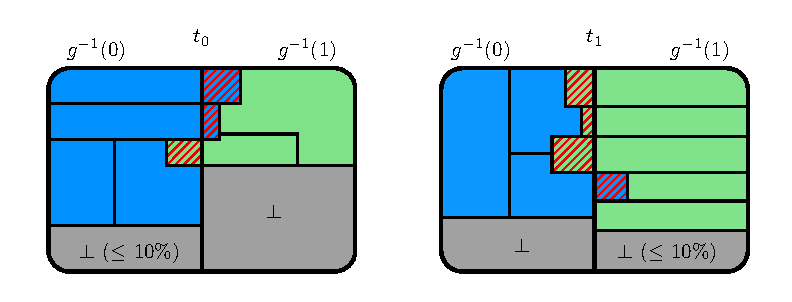
\includegraphics[width=.9\linewidth]{sources/author-figure1.pdf}\end{center}
Figure1. Two trees $t_0$ and $t_1$ in the proof of Hard Side Lemma. The leaves partition $\operatorname{dom}(g)$ into subcubes where grey leaves output $\bot$, green leaves output 1, and blue leaves output 0. Hatched regions are error. We are promised that, e.g., $t_0$ has bounded abort (10\% in our figure) over $\mu^0$, but not necessarily over $\mu^1$.
\paragraph{Tree $t$ errs rarely.} We start with a claim that says that if the expected relative error is low over one side $\mu^b$ of $\mu$, then a $\mu$-smart tree errs rarely over the whole distribution $\mu$.
\begin{authorclaim}{Claim12}
Let $t'$ be $\mu$-smart and $b\in\{0,1\}$. If $\mathbb E_{x\sim\mu^b}[\operatorname{re}(\ell_x^{t'},\mu)]\le\epsilon$ then $\Pr_{x\sim\mu}[t'(x)\text{ errs}]\le\epsilon^{1/2}$.
\end{authorclaim}
\begin{proof}
We prove the claim for $b=0$ as the other case is analogous. Since $t'$ and $\mu$ are fixed, we drop them from notation writing $\operatorname{re}(\ell):=\operatorname{re}(\ell,\mu)$, $\ell_x:=\ell_x^{t'}$, $L:=L(t')$. We argue that relative error on one side of the distribution must spill over to the other side:
\begin{align*}
\mathbb E_{x\sim\mu^0}[\operatorname{re}(\ell_x)]&=\sum_{\ell\in L}\ell(\mu^0)\operatorname{re}(\ell)\ge\sum_{\ell\in L}\ell(\mu^1)\operatorname{re}(\ell)^2\\
&=\mathbb E_{x\sim\mu^1}[\operatorname{re}(\ell_x)^2]\ge\mathbb E_{x\sim\mu^1}[\operatorname{re}(\ell_x)]^2.
\end{align*}
Here the first inequality used $\ell(\mu^0)\ge\ell(\mu^1)\operatorname{re}(\ell)$ (from Claim11) and the second inequality used Jensen's inequality. It follows that $\mathbb E_{x\sim\mu^1}[\operatorname{re}(\ell_x)]\le\mathbb E_{x\sim\mu^0}[\operatorname{re}(\ell_x)]^{1/2}\le\epsilon^{1/2}$ and therefore $\mathbb E_{x\sim\mu}[\operatorname{re}(\ell_x)]\le\epsilon^{1/2}$. The claim then follows from Claim10.
\end{proof}
We now verify property(6), which concludes the proof of Hard Side Lemma.
\begin{align*}
\Pr_{x\sim\nu}[t(x)\text{ errs}]&\le\Pr_{x\sim\nu}[t_0(x)\text{ errs}\vee t_1(x)\text{ errs}]\\
&\le\sum_{b\in\{0,1\}}\Pr_{x\sim\nu}[t_b(x)\text{ errs}]\\
&=\sum_{b\in\{0,1\}}\lambda\Pr_{x\sim\mu^0}[t_b(x)\text{ errs}]+(1-\lambda)\Pr_{x\sim\mu^1}[t_b(x)\text{ errs}]\\
&\le\sum_{b\in\{0,1\}}2\Pr_{x\sim\mu}[t_b(x)\text{ errs}]\le\sum_{b\in\{0,1\}}2\cdot\epsilon^{1/2}\quad\text{(Claim12 and(8))}\\
&=4\epsilon^{1/2}\le\epsilon^{1/3}.\quad(\epsilon\ll1)
\end{align*}

% Faithful formal-publication transcription: complete Section5.
\section*{5 Proof of Multileaf Lemma}
\begin{authorclaim}{Multileaf Lemma (restated)}
For every partial $g$ and $0<\epsilon\lll\delta\ll1$, there exists a distribution $\mu=\frac12(\mu^0+\mu^1)$ over $\operatorname{dom}(g)$ and a hard side $b\in\{0,1\}$ such that for every deterministic tree $t$ taking inputs from $\operatorname{dom}(g^n)$ and having $\operatorname{depth}(t)/(n\overline R_\epsilon(g))\lll\delta$,
\[\forall y\in\{0,1\}^n:\quad\Pr_{x\sim\mu^y}[\ell_x^t\text{ is }(\delta,\epsilon,\mu,b)\text{-noisy}]\ge1-\delta.\]
\end{authorclaim}
\begin{proof}
Apply Leaf Lemma with parameters $\epsilon$ and $\dot\delta:=\delta^3$ (assuming suitably $0<\epsilon\lll\dot\delta\ll1$) to obtain $\mu=\frac12(\mu^0+\mu^1)$ and $b\in\{0,1\}$ that satisfy the lemma for trees of depth at most $\dot\delta^c\overline R_\epsilon(g)$. Fix $y\in\{0,1\}^n$ and a deterministic tree $t$ over $\operatorname{dom}(g^n)$ with $\operatorname{depth}(t)\le\dot\delta^{c+4}n\overline R_\epsilon(g)$ (where we chose $3(c+4)$ as the exponent hidden by $\lll$).
Here is the plan for our proof. An input $x\in\operatorname{dom}(g^n)$ can be seen as inducing several subtrees of $t$ corresponding to distinct coordinates $i\in[n]$. Indeed, define $t_{x,i}$ as the tree over inputs from $\operatorname{dom}(g)$ that is obtained from $t$ by substituting $x$ as its input variables except retaining $x_i$ as free variables. If we can show that $t_{x,i}$ has shallow depth in expectation over an input $z\sim\mu^{y_i}$ then we can hope to use and argue that the reached leaf $\ell_z\in L(t_{x,i})$ (which is one of the $n$ components of a leaf of $t$) is typically $(\epsilon,\mu,b)$-noisy.
Let us formalise this plan. Let $x\sim\mu^y$ henceforth. For $i\in[n]$ we define two events
\begin{align*}
\text{$i$-th tree is shallow: }\quad S_i(x)&\Longleftrightarrow\mathbb E_{z\sim\mu^{y_i}}[q(t_{x,i},z)]\le\dot\delta^c\overline R_\epsilon(g),\\
\text{$i$-th leaf is noisy: }\quad N_i(x)&\Longleftrightarrow\ell_{x_i}\in L(t_{x,i})\text{ is }(\epsilon,\mu,b)\text{-noisy}.
\end{align*}
Note that Leaf Lemma states $\Pr_x[N_i\mid S_i]\ge1-\dot\delta$. Thinking of $S_i$ and $N_i$ as indicator variables, we define $S:=\frac1n\sum_iS_i$ and $N:=\frac1n\sum_iN_i$. With this notation, Multileaf Lemma becomes equivalent to
\begin{equation}\tag{9}\Pr_x[N\ge1-\delta]\ge1-\delta.\end{equation}
To show this, we compute as follows (using Claim13 that is proved below)
\begin{align*}
\mathbb E_x[N]&=\frac1n\sum_i\Pr_x[N_i]\ge\frac1n\sum_i(1-\dot\delta)\Pr[S_i]\quad\text{(Leaf Lemma)}\\
&=(1-\dot\delta)\mathbb E_x[S]\ge(1-\dot\delta)(1-\dot\delta)\quad\text{(Claim13)}\\
&\ge1-\delta^2.\quad(\dot\delta:=\delta^3\ll1)
\end{align*}
Hence(9) follows by applying Markov's inequality to the nonnegative random variable $1-N\ge0$. This completes the proof apart from the following claim.
\end{proof}
\begin{authorclaim}{Claim13}
$\mathbb E_x[S]\ge1-\dot\delta$.
\end{authorclaim}
\begin{proof}
Let $q_i(t,x)$ denote the number of queries made by $t$ to the $i$-th component of $x$. Define $x^{i\leftarrow z}$ as a copy of $x$ but where $z$ is inserted at the $i$-th component. Note that $q_i(t,x^{i\leftarrow z})=q(t_{x,i},z)$. Linearity of expectation gives
\begin{equation}\tag{10}\sum_{i\in[n]}\mathbb E_x[q_i(t,x)]\le\operatorname{depth}(t)\le\dot\delta^{c+4}n\overline R_\epsilon(g).\end{equation}
Define $I\subseteq[n]$ as the set of coordinates $i$ satisfying
\begin{equation}\tag{11}\mathbb E_x[q_i(t,x)]\le\dot\delta^{c+2}\overline R_\epsilon(g).\end{equation}
We have that $|I|\ge(1-\dot\delta^2)n$ as otherwise more than $\dot\delta^2n$ terms in the sum(10) are larger than $\dot\delta^{c+2}\overline R_\epsilon(g)$ contradicting the upper bound on $\operatorname{depth}(t)$. Fix $i\in I$. Sampling $x\sim\mu^y$ is equivalent to first taking $x\sim\mu^y$, then sampling independently $z\sim\mu^{y_i}$, and finally outputting $x^{i\leftarrow z}$. Hence
\[\mathbb E_x\mathbb E_{z\sim\mu^{y_i}}[q_i(t,x^{i\leftarrow z})]=\mathbb E_x[q_i(t,x)]\le\dot\delta^{c+2}\overline R_\epsilon(g).\]
We get from Markov's inequality and the above that
\begin{equation}\tag{12}\Pr_x[\neg S_i]=\Pr_x\left[\mathbb E_{z\sim\mu^{y_i}}[q_i(t,x^{i\leftarrow z})]>\dot\delta^c\overline R_\epsilon(g)\right]\le\dot\delta^2.\end{equation}
In conclusion,
\[\mathbb E_x[S]\ge\frac1n\sum_{i\in I}\Pr_x[S_i]\ge\frac1n|I|\cdot(1-\dot\delta^2)\ge(1-\dot\delta^2)^2\ge1-\dot\delta.\]
\end{proof}

\begin{thebibliography}{25}

\bibitem[1]{ref1}
Anurag Anshu, Dmitry Gavinsky, Rahul Jain, Srijita Kundu, Troy Lee, Priyanka Mukhopad- hyay, Miklos Santha, and Swagato Sanyal. A composition theorem for randomized query complexity. In Proceedings of the 37th Conference on Foundations of Software Technology and Theoretical Computer Science (FSTTCS), pages 10:1–10:13. Schloss Dagstuhl, 2017. doi:10.4230/LIPIcs.FSTTCS.2017.10.

\bibitem[2]{ref2}
Andrew Bassilakis, Andrew Drucker, Mika Göös, Lunjia Hu, Weiyun Ma, and Li-Yang Tan. The power of many samples in query complexity. In Proceedings of the 47th International Colloquium on Automata, Languages, and Programming (ICALP), volume 168, pages 9:1–9:18. Schloss Dagstuhl, 2020. doi:10.4230/LIPIcs.ICALP.2020.9.

\bibitem[3]{ref3}
Shalev Ben-David and Eric Blais. A new minimax theorem for randomized algorithms. In Proceedings of the 61st Symposium on Foundations of Computer Science (FOCS), pages 403–411, 2020. doi:10.1109/FOCS46700.2020.00045.

\bibitem[4]{ref4}
Shalev Ben-David and Eric Blais. A tight composition theorem for the randomized query complexity of partial functions. In Proceedings of the 61st Symposium on Foundations of Computer Science (FOCS), pages 240–246, 2020. doi:10.1109/FOCS46700.2020.00031.

\bibitem[5]{ref5}
Shalev Ben-David, Mika Göös, Robin Kothari, and Thomas Watson. When is amplification necessary for composition in randomized query complexity? In Proceedings of the 22nd International Conference on Randomization and Computation (RANDOM), volume 176, pages 28:1–28:16. Schloss Dagstuhl, 2020. doi:10.4230/LIPIcs.APPROX/RANDOM.2020.28.

\bibitem[6]{ref6}
Shalev Ben-David and Robin Kothari. Randomized query complexity of sabotaged and com- posed functions. Theory of Computing, 14(1):1–27, 2018. doi:10.4086/toc.2018.v014a005.

\bibitem[7]{ref7}
Eric Blais and Joshua Brody. Optimal separation and strong direct sum for randomized query complexity. In Proceedings of the 34th Computational Complexity Conference (CCC), pages 29:1–29:17. Schloss Dagstuhl, 2019. doi:10.4230/LIPIcs.CCC.2019.29.

\bibitem[8]{ref8}
Joshua Brody, Jae Tak Kim, Peem Lerdputtipongporn, and Hariharan Srinivasulu. A strong XOR lemma for randomized query complexity. Technical report, arXiv, 2020. arXiv:2007. 05580.

\bibitem[9]{ref9}
Harry Buhrman and Ronald de Wolf. Complexity measures and decision tree complexity: A survey. Theoretical Computer Science, 288(1):21–43, 2002. doi:10.1016/S0304-3975(01) 00144-X.

\bibitem[10]{ref10}
Chinmoy Dutta and Jaikumar Radhakrishnan. Lower bounds for noisy wireless networks using sampling algorithms. In Proceedings of the 49th Symposium on Foundations of Computer Science (FOCS), pages 394–402. IEEE, 2008. doi:10.1109/FOCS.2008.72.

\bibitem[11]{ref11}
William Evans and Nicholas Pippenger. Average-case lower bounds for noisy boolean decision trees. SIAM Journal on Computing, 28(2):433–446, 1998. doi:10.1137/S0097539796310102.

\bibitem[12]{ref12}
Uriel Feige, Prabhakar Raghavan, David Peleg, and Eli Upfal. Computing with noisy informa- tion. SIAM Journal on Computing, 23(5):1001–1018, 1994. doi:10.1137/S0097539791195877.

\bibitem[13]{ref13}
Dmitry Gavinsky, Troy Lee, Miklos Santha, and Swagato Sanyal. A composition theorem for randomized query complexity via max-conflict complexity. In Proceedings of the 46th International Colloquium on Automata, Languages, and Programming (ICALP), pages 64:1– 64:13. Schloss Dagstuhl, 2019. doi:10.4230/LIPIcs.ICALP.2019.64.

\bibitem[14]{ref14}
Mika Göös, Shachar Lovett, Raghu Meka, Thomas Watson, and David Zuckerman. Rectangles are nonnegative juntas. SIAM Journal on Computing, 45(5):1835–1869, 2016. doi:10.1137/ 15M103145X.

\bibitem[15]{ref15}
Navin Goyal and Michael Saks. Rounds vs. queries tradeoff in noisy computation. Theory of Computing, 6(1):113–134, 2010. doi:10.4086/toc.2010.v006a006.

\bibitem[16]{ref16}
Rahul Jain and Hartmut Klauck. The partition bound for classical communication complexity and query complexity. In Proceedings of the 25th Conference on Computational Complexity (CCC), pages 247–258. IEEE, 2010. doi:10.1109/CCC.2010.31.

\bibitem[17]{ref17}
Rahul Jain, Hartmut Klauck, and Miklos Santha. Optimal direct sum results for deterministic and randomized decision tree complexity. Information Processing Letters, 110(20):893–897, 2010. doi:10.1016/j.ipl.2010.07.020.

\bibitem[18]{ref18}
Stasys Jukna. Boolean Function Complexity: Advances and Frontiers, volume 27 of Algorithms and Combinatorics. Springer, 2012.

\bibitem[19]{ref19}
Jedrzej Kaniewski, Troy Lee, and Ronald de Wolf. Query complexity in expectation. In Proceedings of the 42nd International Colloquium on Automata, Languages, and Programming (ICALP), pages 761–772. Springer, 2015. doi:10.1007/978-3-662-47672-7\_62.

\bibitem[20]{ref20}
Claire Kenyon and Valerie King. On boolean decision trees with faulty nodes. Random Structures and Algorithms, 5(3):453–464, 1994. doi:10.1002/rsa.3240050306.

\bibitem[21]{ref21}
Troy Lee, Rajat Mittal, Ben Reichardt, Robert Špalek, and Mario Szegedy. Quantum query complexity of state conversion. In Proceedings of the 52nd Symposium on Foundations of Computer Science (FOCS), pages 344–353. IEEE, 2011. doi:10.1109/FOCS.2011.75.

\bibitem[22]{ref22}
Ilan Newman. Computing in fault tolerant broadcast networks and noisy decision trees. Random Structures and Algorithms, 34(4):478–501, 2009. doi:10.1002/rsa.20240.

\bibitem[23]{ref23}
Ben Reichardt. Reflections for quantum query algorithms. In Proceedings of the 22nd Symposium on Discrete Algorithms (SODA), pages 560–569. SIAM, 2011.

\bibitem[24]{ref24}
Petr Savický. On determinism versus unambiquous nondeterminism for decision trees. Technical Report TR02-009, Electronic Colloquium on Computational Complexity (ECCC), 2002. URL: http://eccc.hpi-web.de/report/2002/009/.

\bibitem[25]{ref25}
Avishay Tal. Properties and applications of boolean function composition. In Proceedings of the 4th Conference on Innovations in Theoretical Computer Science (ITCS), pages 441–454. ACM, 2013. doi:10.1145/2422436.2422485.
\end{thebibliography}
\end{document}
